\documentclass[a4paper,11pt]{article}
\pagestyle{empty}
\usepackage{amssymb}
\usepackage{amsmath}
\usepackage{graphicx}
\usepackage{graphics}
\usepackage{epstopdf}
\usepackage{color}

\pdfpagewidth 9.75in
\pdfpageheight 12.0in 

\setlength\topmargin{-0.5in}
\setlength\headheight{-0.0in}
\setlength\headsep{0.2in}
\setlength\textheight{10.5in}
\setlength\textwidth{6.75in}
\setlength\oddsidemargin{0in}
\setlength\evensidemargin{0in}
\setlength\parindent{0.1in}
\setlength\parskip{0.25em}


\usepackage{fancyhdr,lastpage}
\pagestyle{fancy}
\fancyhead[L]{}
\fancyhead[R]{}

\newif\ifdraft
%\drafttrue
\ifdraft
\newcommand{\fixme}[1]{ { \bf{ ***FIXME: #1 }} }
\newcommand{\jhanote}[1]{ {\textcolor{red} { ***Jha: #1 }}}
\else
\newcommand{\jhanote}[1]{}
\newcommand{\fixme}[1]{}
\fi

\begin{document}

Case I:

In this scenario, we are examining how data sets are handled
when all operations are local.  The purpose of this case it
rule out factors that could be misleading in distributed
data set experiments.  

There are several variations on this experiment to determine
which factors are exerting themselves.  We first try our
base case to base all other variations off of.  This way we
can change one variable at a time and see how results are
altered.

\includegraphics{figure1.eps}

The small assignment case has more files while keeping the
total data set size the same.  Also, to accommodate these
files, there are more assignments being made.  This means
essentially that there are twice as many files, so there has
to be twice as many work units getting completed.

The large assignment test also has twice as many files as in
the small assignment case, but differs because it puts more
files per work unit, so the work units are the same as in
the base case.

Since there is very little difference between the small and
large assignment cases, we can conclude that changing the
overall number of files is causing the scaling factor, not
the number assignments.  This shows that the overhead is not
caused by the handling of many workers coming in to handle
work units, but by opening the extra files in the worker
case.

Our proposed model is as follows

Ts = ceil(num(workunits) / num(worker)) * (totalDataSizePerWorkunit / readSpeedOfMachine)

This model does not differentiate between number of files
per work unit as just noted above as being significant.
Also, this model does not take into account that as the
number of workers approaches the number of cores on the
machine, we see a slowdown that can not be avoided by adding
more workers. We clearly need a better worker


\end{document}
